%
% $Id: ch03_thework.tex
%
%   *******************************************************************
%   * SEE THE MAIN FILE "AllegThesis.tex" FOR MORE INFORMATION.       *
%   *******************************************************************
%
\chapter{Method of Approach}
\label{ch:methods}

 \name{} was developed using a modified agile approach; short development ``sprints'' were executed for key system development.
We describe the product of some of those sprints in Section~\ref{ch:methods:renderer}, primarily the ray-tracing engines.
In Section~\ref{ch:methods:interface} we also describe the Tickit interface and its algorithms.
The overall structure of the project is twofold: there is an unfinished research prototype, called \texttt{rayterm-cpu}, as well as a finished prototype called \texttt{rayterm-gpu}, or simply \name{}.
We will describe the development process of these implementations further in Chapter~\ref{ch:implementation}; this chapter focuses on the algorithms, design, and overall structure of the project.


\section{Render Engines}
\label{ch:methods:renderer}
While building \name{}, two separate render engine prototypes were implemented.
The first, which we describe in Section~\ref{ch:methods:renderer:sequential}, was a simple, single core sequential renderer~\cite{raytermCpuImpl}.
This engine was developed in three main development sprints, over a period of about two months.
The second, described in Section~\ref{ch:methods:renderer:parallel}, uses CUDA~\cite{nvidia2011cuda} and OptiX~\cite{parker2010optix} to leverage GPU compute power in parallel.
This engine was developed over two sprints, in a little under a month.


\subsection{Sequential}
\label{ch:methods:renderer:sequential}

The sequential renderer, or \texttt{rayterm-cpu}, is a CPU-only ray-tracer.
It supports three different types of materials: diffuse, metallic, and dielectric.
These materials are complemented with two geometric primitives: disks, and spheres.
Figure~\ref{fig:rayterm-cpu_ppm} shows an image of the \texttt{ppm} output of \texttt{rayterm-cpu} near the end of its development.
The Tickit interface was never integrated into the CPU implementation, as this implementation is not performant enough for even simple scenes at low resolution.
For example, Figure~\ref{fig:rayterm-cpu_ppm} was rendered in about twenty seconds on a modern CPU.

\vspace{0.3em}
\begin{figure}[htb]
  \centering
  \includegraphics[width=0.75\textwidth]{impl-images/first_positionable_camera}
  \caption{\texttt{rayterm-cpu} example \texttt{ppm} output}
\label{fig:rayterm-cpu_ppm}
\end{figure}

The main advantage of a sequential renderer is the lower development overhead since there is no need to interface with a complex device such as a GPU.
This means that there is no need for handling parallel execution, and each ray is computed one after the other.
Because of this simplicity, this engine's development was perfectly suited for the goal of gaining knowledge and experience in ray-tracing.
The development also explored many fundamentals so that future contributions would be well-founded.
With 219 commits and over a thousand lines of code in the final product, along with many thousands of additions and deletions, \texttt{rayterm-cpu} accomplished its goals.

\subsubsection{Design}
\label{ch:methods:renderer:sequential:design}

The sequential renderer's design relies on two main components, as well as the Eigen linear algebra library~\cite{eigenweb}.
These components have a linear relationship, as can be seen in Figure~\ref{fig:rayterm-cpu_components}; \texttt{raytrace} deals with tracing rays, \texttt{raymath} with intersection logic, and Eigen with linear algebra.

\vspace{0.3em}
\begin{figure}[htb]
  \centering
  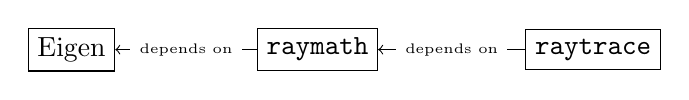
\begin{tikzpicture}
      \node[shape=rectangle,draw=black] (e) at (-3.125,0) {Eigen};
      \node[shape=rectangle,draw=black] (rm) at (0,0) {\texttt{raymath}};
      \node[shape=rectangle,draw=black] (rt) at (3.5,0) {\texttt{raytrace}};

      \path [<-](e) edge node[midway, fill=white] {\tiny depends on} (rm);
      \path [<-](rm) edge node[midway, fill=white] {\tiny depends on} (rt);
  \end{tikzpicture}
  \caption{Component and dependency relationships in \texttt{rayterm-cpu}}
\label{fig:rayterm-cpu_components}
\end{figure}

Eigen~\cite{eigenweb} is a linear algebra for C++ that supports matrix and vector manipulations, various matrix decompositions and geometry features, and has many extensions for numerous other numerical operations.
Eigen is also extremely well-optimized and uses SSE vectorized code, vastly improving performance on supported CPUs.
In \texttt{raymath}, Eigen is used primarily for easy, tested representations and calculations involving vectors; all of the algorithms implemented use equations derived from the ones in Section~\ref{ch:intro:background:raytracing_math}, and so benefit from easy implementation.

The base component in \texttt{rayterm-cpu}\,---\,\texttt{raymath}\,---\,provides support for various geometries and intersection routines.
The geometries supported can be seen in Figure~\ref{fig:rayterm-cpu_raymath_geometry}, and use Eigen structures to represent their geometric data.
\texttt{raymath} also handles random number and vector generation, color handling, and intersection representation.
The implementations behind these are covered in Section~\ref{ch:implementation:prototype:raymath}.

\vspace{0.3em}
\begin{figure}[htb]
  \centering
  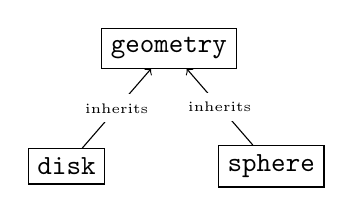
\begin{tikzpicture}
    \node[shape=rectangle,draw=black] (g) at (0,1.5) {\texttt{geometry}};
      \node[shape=rectangle,draw=black] (s) at (1.3,0) {\texttt{sphere}};
      \node[shape=rectangle,draw=black] (d) at (-1.3,0) {\texttt{disk}};

      \path [<-](g) edge node[midway, fill=white] {\tiny inherits} (s);
      \path [<-](g) edge node[midway, fill=white] {\tiny inherits} (d);
  \end{tikzpicture}
  \caption{Geometric structures in \texttt{raymath}}
\label{fig:rayterm-cpu_raymath_geometry}
\end{figure}

The main component in \texttt{rayterm-cpu} is \texttt{raytrace}; it handles world representation, materials, and ray-tracing.
\texttt{rayterm-cpu} only renders in \texttt{ppm} mode, since the Tickit interface was only integrated in the \texttt{rayterm-gpu} implementation, since that was the final prototype.
\texttt{raytrace} represents objects with a \texttt{WorldObject} class, a list of which is stored in a \texttt{World}.

Figure~\ref{fig:rayterm-cpu_raytrace_journey_of_a_ray} shows the function call path that is used when rendering a single ray.
The main entry point is \texttt{raytrace\_ppm}, which creates rays with a \texttt{Camera} class instance.
This instance contains specific parameters to control the position and orientation of the virtual camera, and thus controls where the \texttt{ray} originates from, as well as its direction.
Then, that \texttt{ray} is sent on to the \texttt{World} class, where an \texttt{intersection} is retrieved, and then used to generate a \texttt{color} from the given \texttt{ray}.
This color is then finally returned to \texttt{raytrace\_ppm}, which writes it to a \texttt{ppm} file.
Unmentioned in this diagram are the recursive calls to \texttt{World::trace} from from \texttt{WorldObject::colorize}, which use the transformed ``scatter'' \texttt{ray} from \texttt{Material::scatter}.
The implementation behind all of these structures and functions are covered in Section~\ref{ch:implementation:prototype:raytrace}.

\vspace{0.3em}
\begin{figure}[htb]
  \centering
  \begin{tikzpicture}
    \node[shape=rectangle, draw=black] (a) at (0,0) {Ray collection (\texttt{raytrace\_ppm})};
    \node[shape=rectangle, draw=black, right = 2.25em of a ] (b) {Generation (\texttt{Camera::get\_screen\_ray})};
    \node[shape=rectangle, draw=black, below = 1.75em of a] (c) {World tracing (\texttt{World::trace})};
    \node[shape=rectangle, draw=black, right = 2.25em of c] (e) {Ray coloring (\texttt{WorldObject::colorize})};
    \node[shape=rectangle, draw=black, below = 1.75em of e] (s) {Ray scattering (\texttt{Material::scatter})};
    \node[shape=rectangle, draw=black, below = 1.75em of c] (d) {World intersection (\texttt{World::intersects})};
    \begin{scope}[xshift=1cm]
      \node[shape=rectangle, draw=black] (f) at (2.75, -4.15) {Object intersection (\texttt{WorldObject::intersects})};
      \node[shape=rectangle, draw=black, below = 1.75em of f] (g) {Geometry intersection (\texttt{geometry::intersects})};
      \path [->](d) edge node[midway, fill=white] {\tiny calls} (f);
      \path [->](f) edge node[midway, fill=white] {\tiny calls} (g);
    \end{scope}

      \path [->](a) edge node[midway, fill=white] {\tiny calls} (b);
      \path [->](a) edge node[midway, fill=white] {\tiny calls} (c);
      \path [->](c) edge node[midway, fill=white] {\tiny calls} (d);
      \path [->](c) edge node[midway, fill=white] {\tiny calls} (e);
      \path [->](e) edge node[midway, fill=white] {\tiny calls} (s);
  \end{tikzpicture}
  \caption{The journey of a \texttt{ray} and its \texttt{intersection}}
\label{fig:rayterm-cpu_raytrace_journey_of_a_ray}
\end{figure}

\subsubsection{Algorithms}
\label{ch:methods:renderer:sequential:algorithms}

The sequential renderer implements single-branch Monte Carlo ray-tracing, a type of rendering that can produce physically accurate images with little development effort.
The algorithm is largely based on randomness, only modifying the path of a single ray at a time as it bounces around the scene.
When encountering objects, a particular Probability Distribution Function (PDF) is used to calculate where the ray will bounce.
These PDFs vary based on the material and are hard-coded in the \texttt{Material} implementation.
The result of this algorithm is extremely noisy because of this randomness (see Figure~\ref{fig:rayterm-cpu_ppm_noisy}), so many samples must be taken and then averaged to gain a true value for a single pixel; this simulates the many millions of photons that would have traveled to that pixel in a real camera.
The number of samples per pixel, sometimes termed ``spp,'' is the number of rays generated from a random origin within the pixel; this is done for every pixel in the image.
An example of various spp values is shown in Figure~\ref{fig:rayterm-cpu_ppm_noisy}.

\vspace{0.3em}
\begin{figure}[htb]
  \centering
  \begin{subfigure}[htb]{0.45\textwidth}
    \includegraphics[width=\textwidth]{impl-images/comparisons/samples_spp_1}
    \caption{1 sample per pixel}
\label{fig:rayterm-cpu_ppm_noisy_1}
  \end{subfigure}
  \hspace{1em}
  \begin{subfigure}[htb]{0.45\textwidth}
    \includegraphics[width=\textwidth]{impl-images/comparisons/samples_spp_4}
    \caption{4 samples per pixel}
\label{fig:rayterm-cpu_ppm_noisy_4}
  \end{subfigure}
  \vspace{1em}
  \begin{subfigure}[htb]{0.45\textwidth}
    \includegraphics[width=\textwidth]{impl-images/comparisons/samples_spp_32}
    \caption{32 samples per pixel}
\label{fig:rayterm-cpu_ppm_noisy_32}
  \end{subfigure}
  \hspace{1em}
  \begin{subfigure}[htb]{0.45\textwidth}
    \includegraphics[width=\textwidth]{impl-images/comparisons/samples_spp_1024}
    \caption{1024 samples per pixel}
\label{fig:rayterm-cpu_ppm_noisy_1024}
  \end{subfigure}
  \caption{Sample per pixel differentiated output from \texttt{rayterm-cpu}}
\label{fig:rayterm-cpu_ppm_noisy}
\end{figure}

For an spp value of four, there are four rays generated for each pixel; thus, the rendering equation~\cite{kajiya1986rendering} is approximated at the first intersection by four random direction samplings (keep in mind the integration is over the sphere or hemisphere around the point of intersection for each ray).
Thus, the more rays generated, the more accurate that sampling becomes.
This is still not really solving the rendering equation and is a large simplification.
Rather, the different eye-rays generated because of the spp value sample slightly different intersection points.
These rays then also sample different directions out of those intersection points, and so are a kind of ``fuzzy'' approximation.
An area for future work is implementing a kind of ``stratification'' of these samples, so that they are not randomly spread, but instead fully sample the sphere or hemisphere at a certain resolution;
This would likely be combined with branched Monte Carlo rendering, which involves generating multiple rays for each intersection hit, thereby actually sampling the same integral.
This would reduce the noise at low spp values significantly better than simply increasing the spp value, although at the slight cost of performance (more rays to calculate).

\noteworthy{
  N_{ops} = R \cdot S \cdot D \cdot N
}{Ray-tracing Operations}

In discussing the complexity of this implementation, there are four main variables to keep in mind: first, the number of pixels to render, $R$; second, the number of samples per pixel, $S$; third, the maximum number of recursions per sample, $D$; and fourth, the number of intersectable objects in the scene, $N$.
The number of pixels to render varies with the resolution of the desired image.
The number of samples per pixel and the maximum number of recursions are both user-specified configurable values.
The number of objects in the scene can vary wildly, but most test scenes in \texttt{rayterm-cpu} have less than $10$ objects.
This gives us Formula~\ref{Ray-tracing Operations} to calculate the number of base ``ray tracing operations'' which we call $N_{ops}$.
These operations consist of a single ray-tracing intersection operation, which involves testing a ray against a single parametric equation for intersection.
As long as that operation can be considered constant, $O(R \cdot S \cdot D \cdot N)$ is the time complexity of the Monte Carlo algorithm used in \texttt{rayterm-cpu}.
For spheres and disks, the only geometry supported, the intersection routine depends on both $sqrt()$ and $dot()$.
However, the time complexities of these functions probably do not vary with respect to the value given to them.
For taking the square root, there is likely system support for fast calculation independent of the input value; for vector dot products, the size is always constant at three entries.
Because of this, we can consider the time complexity of a single intersection test to be constant.
Thus, the time to complete a render varies proportionally to the number of objects in the scene, the resolution of the image, the number of samples per pixel, and the ray-tracing depth.

As an example, take a scene with $3$ spheres and a disk.
Let us render an $80$ by $52$ pixel image;
we will choose to use $32$ samples per pixel to get a reasonable image quality.
For maximum recursion depth, a value of $5$ should be plenty for the simple scene we have\,---\,a more complex scene could probably benefit from a few more, but since attenuation reduces the impact each successive ray has on a fragment, it is very unlikely to matter past a few tens.
Thus, we have all the information we need: $R = 4160,\ S = 32,\ D = 5,\ N = 4$.
We can calculate the final number of basic ray-tracing intersections by simply multiplying these variables together: we get $2662400$.
Since this kind of image can usually be rendered in around 200 milliseconds by \texttt{rayterm-cpu}, we can get a sense of how fast the existing intersection is already: one test takes about $75$ nanoseconds.
There's not much hope of drastically improving this time.
Even to get render time down to $33$ milliseconds, which is needed for $30$ frames per second playback, we would need an intersection test to take no more than $12.4$ nanoseconds.
This is nigh impossible with modern CPUs\,---\,for comparison, basic multiplication takes an average 19 nanoseconds on an i7-4770k, a relatively modern processor\,---\,the code to calculate this value on any computer can be seen in Appendix~\ref{appendix:timemul}.
Therefore any further major performance improvement needs to break out of the sequential world this algorithm was written in.

The algorithms used for object intersection are already covered in Section~\ref{ch:intro:background:raytracing_math}; however the scattering algorithms are discussed below.
There are three materials supported in \texttt{rayterm-cpu}: Lambertian, metallic, and dielectric.
The Lambertian material, sometimes known as diffuse, is very simple; the scattered ray originates at the intersection location, and the direction is random in the unit hemisphere oriented about the surface normal of the intersected object.
Essentially, when a ray hits a Lambertian object the ray reflects around the tiny crevices and cracks on the surface of the object so that the direction is entirely random once it leaves the object.

\noteworthy{
  \vec{R_{reflect}} = \vec{R_{in}} - 2(\vec{S_{normal}} \bullet \vec{R_{in}})\vec{S_{normal}}
}{Ray Reflection}

The metallic material scatters rays in a similar way as the Lambertian but includes a bias towards the reflection direction.
The reflection direction is calculated using Formula~\ref{Ray Reflection}~\cite{prunier2017shading}, where $\vec{R_{reflect}}$ is the reflected ray, $\vec{R_{in}}$ is the incoming ray, and $\vec{S_{normal}}$ is the surface normal.
The bias is generated by using a ray direction that is linearly interpolated between the pure reflection direction from Formula~\ref{Ray Reflection} and a random direction generated as in Lambertian materials.
The amount of linear interpolation is known as the ``roughness''\,---\,a roughness of zero gives perfect reflection (a mirror), whereas a roughness of one gives the same results as a Lambertian material.
A slightly more accurate roughness ramp could be attained by using spherical linear interpolation, however, because of the significant performance penalty that was not used.

Finally, the dielectric material is the most complicated.
A dielectric material supports both reflection (as in the other materials), and refraction.
Since we scatter only one ray at a time, the scatter function uses probability to determine which kind of trajectory will be used.
This probability is based on Schlick's approximation of the Fresnel factor, as seen in Formula~\ref{Schlick's Approximation}~\cite{schlick1994inexpensive, learnopengltheory, prunier2017shading}.
In this approximation, $\theta$ is the angle between the incoming ray direction and the surface normal; $n_1$ and $n_2$ are the indices of refraction of the object and air\,---\,these are reversed if the ray is leaving the object.
Finally, $R_0$ is the value of the Fresnel term when there is minimal reflection \textit{i.e.} when $\theta = 0$.

\noteworthy{
  R_0 = (\frac{n_1 - n_2}{n_1 + n_2})^2
}{Schlick's Reflection Coefficient}

\noteworthy{
  R(\theta) = R_0 + (1 - R_0)(1 - \cos{\theta})^5
}{Schlick's Approximation}

This approximation gives values close to $0$ when the view angle is high, for example when looking directly through an object; it gives values close to $1$ when the view angle is low, for example on the oblique sides of a sphere.
This can be seen in Figure~\ref{fig:rayterm-cpu_fresnel}: notice that the gradient is not linear and the white is mostly concentrated on the oblique edges of the sphere.
The approximation is then used to determine if the ray will be refracted (low values) or reflected (high values) by testing against a random scalar in the interval $\left[0, 1\right)$.
This will result in high viewing angles (black in Figure~\ref{fig:rayterm-cpu_fresnel}) generating refraction rays, and low viewing angles (white in Figure~\ref{fig:rayterm-cpu_fresnel}) generating reflection rays.
This is a close approximation of the effect that glass and other dielectrics have when viewed in the real world.

\vspace{0.3em}
\begin{figure}[htb]
  \centering
  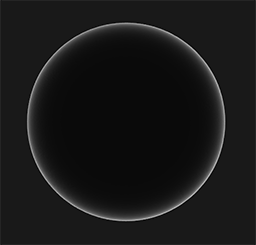
\includegraphics[width=0.4\textwidth]{resources/fresnel}
  \caption{Schlick approximation for a sphere (white is $1$, black is $0$)~\cite{learnopengltheory}}
\label{fig:rayterm-cpu_fresnel}
\end{figure}

Now that the kind of ray has been chosen, the refraction or reflection direction is calculated.
There is an additional possibility that the specific ray we have cannot be refracted because of total internal reflection\,---\,in this case, we switch over to a reflection ray.
The ray direction in the reflection case is calculated with Formula~\ref{Ray Reflection} as in previous materials.
The ray direction in the refraction case is calculated with Formula~\ref{Ray Refraction}.
In this formula, $\eta = \frac{n_{from}}{n_{to}}$ where $n_{from}$ is the index of refraction of the medium we are transferring from and $n_{to}$ is the corresponding index.
Additionally, $I = (\vec{R_{in}} \bullet \vec{S_{normal}})$ where $\vec{R_{in}}$ is the incoming ray and $\vec{S_{normal}}$ is the surface normal.
Finally, $\vec{R_{refract}}$ is the refracted ray.
There is some additional handling in the implementation of this formula to ensure both ray directions (exiting and entering an object) are supported.
This involves flipping the $n$ values and negating $I$ or $\vec{S_{normal}}$.
This formula is derived from the excellent ``Scratchapixel''~\cite{prunier2017shading} and ``Raytracing in One Weekend''~\cite{shirley2016ray}, with some significant rewriting.

\noteworthy{
  \vec{R_{refract}} = \eta\vec{R_{in}} + (\eta I - \sqrt{1 - \eta^2 \cdot (1 - I^2)})\vec{S_{normal}}
}{Ray Refraction}

\subsubsection{Outcome}
\label{ch:methods:renderer:sequential:outcome}

The sequential renderer is only a research prototype and was never finished.
This is primarily because more performance was needed for the final \name{} implementation; the parallel renderer fulfills that need.
Because of the prototype nature of \texttt{rayterm-cpu}, the final implementation only renders images through a Google Test~\cite{googletest} case, which can be run with the \texttt{test.sh} script in the implementation repository~\cite{raytermCpuImpl}, or with \texttt{gradle test}.
This generates a \texttt{test\_image.ppm} file, examples of which we show from various stages of development in Section~\ref{ch:implementation:prototype:raytrace}.
Because of this, \texttt{rayterm-cpu} is very much a proof-of-concept and learning example, rather than a fully-fledged library.

That is not to say that \texttt{rayterm-cpu} was not a useful system.
Many of the algorithms implemented carry over to the parallel renderer, and so the development of that version was aided by existing work.
An excellent example of this is the random generation in \texttt{raymath} and the material scatter functions in \texttt{raytrace}; these algorithms are core to ray-tracing and having a prior implementation simplified further development.
Although they may not carry over unmodified, they are the first iteration in a long improvement cycle.

\subsection{Parallel}
\label{ch:methods:renderer:parallel}

The parallel render engine, \texttt{rayterm-gpu}, uses a Graphics Processing Unit (GPU) to massively parallelize the raytracing algorithm.
This improves performance dramatically because each eye-ray's children (the result of a collision between an object and a ray) are dependent on only their parent eye-ray.
Thus, the computation of a single pixel's color is completely independent of every other pixel.

A short introduction to NVIDIA GPUs may be useful here; they consist primarily of small units of computation circuitry called ``multiprocessors'' which themselves are controllers for several CUDA cores~\cite{fermi2009nvidia}, distributing workloads.
Multiprocessors work on data and code called ``thread blocks.''
Each individual CUDA core in a multiprocessor executes an individual thread in a thread block.
These CUDA cores execute individual threads on the GPU; they can each handle an individual intersection test, and with thousands of them per GPU, we can easily cut the render time down.
There are many restrictions to code that can run in a CUDA thread; CUDA cores act somewhat like advanced floating point arithmetic computation units.
However, OptiX takes care of much of the device handling and thus can perform some advanced optimizations for the individual cores.
A discussion on the specific hardware used for development and testing is available in Section~\ref{ch:intro:background:hardware}.

With 227 commits and over 1.5 thousand lines of code, along with many thousands of additions and deletions, \texttt{rayterm-gpu} has a good start on its life.
There are many, many more improvements possible, however.
We detail some of them in the context of the larger \name{} implementation in Section~\ref{ch:conclusion:future}.
The implementation repository used for \texttt{rayterm-gpu}~\cite{raytermGpuImpl} is also the same used for \name{} as a whole; thus, while we only describe \texttt{rayterm-gpu} in this section, our discussion here also applies to the final \name{} library.
This section specifically covers the \texttt{raytrace} component of the final \name{} library; Section~\ref{ch:methods:interface} covers the \texttt{rayterm} component.
Both of these are combined into a single \texttt{rayterm.so} library for use by other applications.
An example application is also bundled in the implementation repository~\cite{raytermGpuImpl}, as the \texttt{rtexplore} component.
All of these are discussed in more detail in Section~\ref{ch:implementation:final}.

\subsubsection{Libraries}
\label{ch:methods:renderer:parallel:libraries}

Utilizing the massively parallel computation power of a GPU can be difficult\,---\,in fact, before CUDA's release in 2007, there was no well-defined way to do so programmatically.
CUDA is an API and computing platform that enables massively parallel computations~\cite{nvidia2011cuda}.
A special extension of C++, known as CUDA C/C++, can be compiled with \texttt{nvcc}, a custom LLVM-based C/C++ compiler.
This extension enables library support for GPU accelerated multi-threading, physics, and linear algebra, along with many implementations of common data transformation algorithms.
A significant limitation, especially for ray-tracing, is that performance can be significantly affected for inherently divergent tasks\,---\,tasks which do not consistently follow the same control flow\,---\,such as traversing an acceleration structure.

OptiX is an API interface developed for current generation NVIDIA GPUs that enables GPU accelerated ray-object intersection calculations in a programmable pipeline~\cite{parker2010optix, nvidia2019optixdoc}.
It does this by building on top of the CUDA platform, adding abstract and algorithm implementations for common ray-tracing tasks.
OptiX allows user-defined single-ray programs to be compiled into a single program, called a ``kernel,'' that runs on the GPU.
These user programs are written in C++ and then transpiled to PTX, an instruction set for general purpose parallel programming.
Other useful algorithms are also included in the OptiX library, such as BVH and similar acceleration structure implementations.
The main method of communication between host (CPU) and device (GPU) are \texttt{Buffer}s, which are simply arrays managed by OptiX.
Depending on the type of \texttt{Buffer}, data could be moved in one direction or both, depending on the context; an example of this would be the pixel buffer, which is written to on the device and then loaded into CPU-accessible memory for display.

\subsubsection{Programmability}
\label{ch:methods:renderer:parallel:program}

Both OptiX and \name{} itself support programmability in some form.
We will define programmability as the possibility of using user-specified code in some operational capacity at certain points in the program's execution.
For example, it is possible in OptiX to define a CUDA function that will be executed to test if a ray intersects with an object; this enables part of the capability to render any intersectable object with OptiX.
 \name{} supports material programs that are passed on to OptiX to deal with material scatters; because of this it should one day be possible to use NVIDIA MDL materials~\cite{nvidia2015mdl} in \name{}.
We utilize programmability in OptiX in a fairly generic way, because much of the implementation burden for a specific application lies on the application author, and \name{} simply provides an interface.
Before we describe \name{}'s approach, let us consider Figure~\ref{fig:rayterm-gpu_optix_trace}.

\vspace{0.3em}
\begin{figure}[htb]
  \centering
  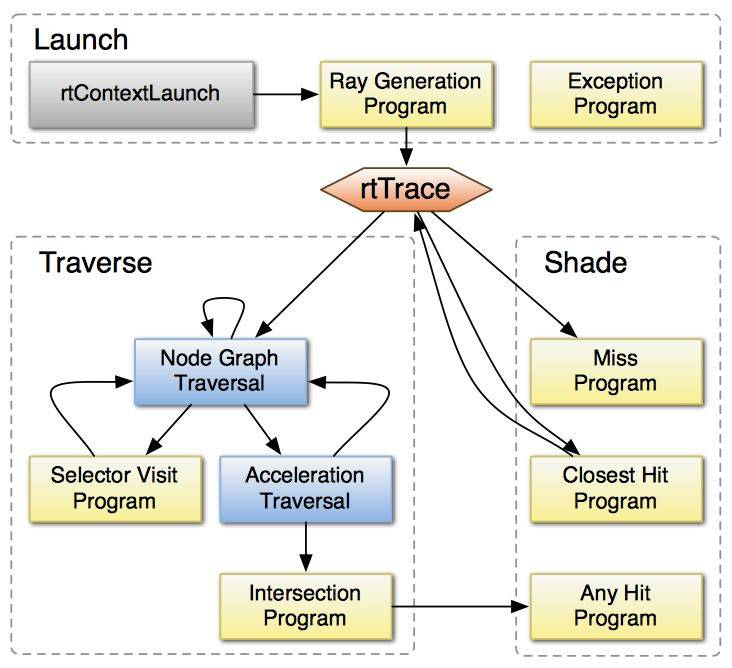
\includegraphics[width=0.7\textwidth]{resources/optix_trace}
  \caption{OptiX Program call graph}
\label{fig:rayterm-gpu_optix_trace}
\end{figure}

In \name{}, we visit only part of Figure~\ref{fig:rayterm-gpu_optix_trace}\,---\,the ``Traverse'' section is not used when RTX mode is enabled: instead, custom intersections and acceleration structures are used for better performance.
In \texttt{rayterm-gpu}, only triangle intersections are supported, and acceleration structure calculations are handed off to OptiX's ``Trbvh'' algorithm~\cite{karras2013fast}.
Triangle intersection and acceleration structure builds are highly optimized in OptiX, more so than any user library could achieve.
In newer NVIDIA RTX GPUs these constraints also enable real hardware acceleration, as opposed to GPU accelerated computation.
In Figure~\ref{fig:rayterm-gpu_optix_trace}, yellow boxes are user-defined programs.
 \name{} defines the Ray Generation Program as a pinhole camera model.
The Exception Program is also defined, with switches to only enable debug prints and exception handling if \name{} is compiled in debug mode.
Lastly, \name{} defines the Miss Program to shade the background of the scene a smooth sky gradient.
The Closest Hit and Any Hit Programs, however, are completely user-defined.
These programs control the scattering of rays when they encounter an object.
How \name{} handles the pass-through configuration of these programs is detailed in the next section.

\name{} supports three asset types: triangle models in the \texttt{OBJ} file format, material definitions in a custom format, and CUDA functions transpiled to PTX, all from arbitrary locations on disk.
These locations are currently specified as compile-time defines \texttt{PROGRAM\_DIRECTORY} and \texttt{ASSET\_DIRECTORY}.
When \name{} or a user application requests a CUDA function, material definition, or object model, these directories are used to search for and load the requested data, which is then inventoried and given an id that the user can reference it with.
This enables easy asset reuse and configurable definition.


\subsubsection{Configurability}
\label{ch:methods:renderer:parallel:config}

At the time of writing, \name{}'s test scene is hard-coded in the \texttt{raytrace} component.
However, it is trivial to provide a loading mechanism so that user applications can specify the scene and any changes to it.
Although the scene itself cannot currently be configured, a wide array of possibilities are available for material and object definitions.
Objects are loaded from an \texttt{OBJ} model file, which should specify at minimum the vertices and vertex normals of the model.
 \name{} uses TinyObjLoader~\cite{tinyobjloader} to load and triangulate \texttt{OBJ} files.
Then, the basic attributes\,---\,vertex positions, normals, shapes, etc.\,---\,are stored in a \texttt{Mesh} object that is inventoried in the resource system.
For materials, a similar process is implemented.
First, a custom parser decodes the given material file, which should conform to the format specified below.
Then, an OptiX \texttt{Material} is created and inventoried.
Finally, the resource system is capable of generating an OptiX \texttt{GeometryInstance}, which links a material and an OptiX \texttt{GeometryTriangles} generated from \texttt{Mesh} data.
This \texttt{GeometryInstance} can then be added to the scene graph and rendered.

\vspace{0.3em}
\begin{figure}[htb]
\centering
\begin{mdframed}[nobreak=true,align=center,userdefinedwidth=30em]
\begin{verbatim}
closest:diffuse,closest_hit,0
any:diffuse,any_hit,0
attrib:diffuse,triangle_attributes
var:float3,varAttenuation,0.15,0.86,0.21
\end{verbatim}
\end{mdframed}
\vspace{-0.3em}
\caption{Sample material definition}
\label{fig:rayterm-gpu_material_def}
\end{figure}

In Figure~\ref{fig:rayterm-gpu_material_def} a sample material definition is shown.
The format of a material definition follows a simple pattern: each line is a single ``command,'' the type of which is determined by the element before the first `\texttt{:}'.
There are four types of commands: \texttt{closest}, \texttt{any}, \texttt{attrib}, and \texttt{var}.
The \texttt{closest} command specifies a CUDA function to use for the Closest Hit Program.
It has the format \texttt{closest:<file\_name>,<function\_name>,<ray\_type>}.
The \texttt{any} command is similar, except that it specifies the Any Hit Program.
The \texttt{attrib} command sets the attribute program for the \texttt{GeometryTriangles} instance this material is eventually paired with; it operates on all ray types, and thus does not need a specifier.
Finally, the \texttt{var} command specifies a variable to pass through to the GPU CUDA function; the format is \texttt{var:<type>,<name>,<value>}.
The possible types are \texttt{int} to \texttt{int4}, and \texttt{float} to \texttt{float4}; the values are specified in a comma-separated list.
In Figure~\ref{fig:rayterm-gpu_material_def}, a variable named \texttt{varAttenuation} is defined as $\vec{(0.15,\ 0.86,\ 0.21)}$.
This variable is used in the \texttt{diffuse} PTX file as the color to attenuate the recursively traced ray by\,---\,it is the color of the object this material is applied to.
Any number of commands are allowed, and any later commands will overwrite previous commands if they contain similar information, such as an attrib command.
There is not currently a way to programmatically generate a \texttt{Mesh} or \texttt{Material}, however, these are possible future improvements to \name{}.

% TODO: explain scene description language here (after it is implemented)

\subsubsection{Design}
\label{ch:methods:renderer:parallel:design}

OptiX is heavily utilized in \texttt{rayterm-gpu}.
Much of the \texttt{raytrace} component deals with initializing and configuring the OptiX context correctly.
The main class is \texttt{Renderer}\,---\,it represents a render engine, and has state about the world and everything in it.
\texttt{Renderer} is designed to be a singleton, although no code in \name{} assumes this; rather, each instance requires its own OptiX context.
This could be a problem: according to the OptiX Programming Guide, ``multiple contexts can be active at one time in limited cases, but this is usually unnecessary.''
In that quote, ``limited cases'' really mean that it is untested and not well supported, although technically possible~\cite{nvidia2019optixdoc}.
So depending on future OptiX changes, multi-renderer programs may or may not be a possibility.

A \texttt{Renderer} has three main components that operate on the OptiX context associated with the instance.
The \texttt{Camera} member instance controls the current view of the world and can be used to translate or rotate that view.
The \texttt{Programs} member instance holds an inventory of loaded OptiX CUDA functions and can be used to load more or get existing ones.
Finally, the \texttt{Resources} member instance holds an inventory of \texttt{Material}s and \texttt{Mesh}s; it can also load more or associate existing assets together to produce \texttt{GeometryInstance}s, which could be added to the OptiX scene graph.
There are other smaller supporting classes, such as \texttt{PixelBuffer}, which helps wrap existing OptiX functionality to ensure safe usage.

\subsubsection{Algorithms}
\label{ch:methods:renderer:parallel:algorithms}

The parallel renderer uses many of the same algorithms as \texttt{rayterm-cpu}, so the previous discussion of those still apply.
There are a few new algorithms that are unique to \texttt{rayterm-gpu}, however.
First, a modification of the pinhole camera model was made.
This was inspired by the camera models available in the advanced OptiX samples~\cite{optixsamples}, and simply rewrites the equations used before in terms of $\phi$ and $\theta$, as polar coordinates.
In this new \texttt{Camera}, $\phi$ represents the rotation about the vertical world axis, and $\theta$ the rotation about the horizontal axis.
This enables easier viewing modification so that the look direction can be controlled with just two control axis.
Second, the color output space is transformed into BT.709~\cite{ituBT709}; this ensures color accuracy and gamma correctness, as well as being the assumed color space for \texttt{ppm} files.


\noteworthy{
  L = \left\{
              \begin{array}{ll}
                \frac{V}{4.5} & \quad V < 0.081 \\
                (\frac{V + 0.099}{1.099})^\frac{1}{0.45} & \quad V \geq 0.081
              \end{array}
    \right.
}{BT.709 Conversion}

Formula~\ref{BT.709 Conversion} shows the piecewise function definition for conversion between a raw color value $V$ and a luminance component $L$.
This is done for each color component to get the final color for each pixel.
Additional algorithms also had to be developed as replacements for CPU-based algorithms in CUDA functions.
For example, a \texttt{drand48} implementation is provided for CUDA functions to use, since the existing implementation is CPU-only.
The implementation directly mirrors the UNIX specification for \texttt{drand48}~\cite{drand48UNIX}.
Additionally, the sampling algorithms based off of \texttt{drand48} were replaced with analytical solutions, to prevent sample looping and provide better uniform distribution.
The math behind the analytical solution is based on resources from ``Scratchapixel'' as well as an older paper by the same author as ``Raytracing in One Weekend''~\cite{prunier2017global, shirley1997map}.
We also use an OptiX provided sampler, \texttt{cosine\_sample\_hemisphere}, to generate the initial sample; the further analytical solution simply transforms that sample to the correct normal space.

\noteworthy{
  N_{interpolated} = B_{x} \vec{N_{1}} + B_{y} \vec{N_{2}} + (1 - B_{x} - B_{y}) \vec{N_{0}}
}{Interpolated Normal}

Finally, we use an algorithm to calculate the interpolated shading normal.
This is very loosely derived from the OptiX samples~\cite{optixsamples}, and uses the default \texttt{GeometryTriangles} attribute program to calculate the barycentric coordinates of the intersection point.
Formula~\ref{Interpolated Normal} shows the calculation for obtaining the interpolated normal; this result is normalized and can then be used for reflection or refraction calculations.
An interpolated value is extremely useful because it takes into account the normals of each individual vertex and attempts to ``smooth'' the shape approximated by the triangle, thus making shading more accurate despite the physical differences.
In Formula~\ref{Interpolated Normal}, $N_{i}$ is the vertex normal of the $i$-th vertex in the triangle, and $B$ is the two dimensional barycentric coordinate of the intersection point.
The calculated result, $N_{interpolated}$, is the smoothed normal.
This smoothing can be disabled by using an \texttt{OBJ} model that has had its normals exported as ``flag''\,---\,this causes each triangle's vertices to have their normals all match the face normal, instead of having individual normals.
This is useful for flat faces since the interpolated normal is then simply the same as the face normal.
Figure~\ref{fig:rayterm-gpu_smooth_normal_comparison} shows a comparison between smoothed normals and face normals (sometimes called ``geometric normals'').
Larger versions of these images are available in Appendix~\ref{appendix:large_figures} as Figure~\ref{fig:rayterm-gpu_smooth_normal_comparison_large}

\vspace{0.3em}
\begin{figure}[htb]
  \centering
  \begin{subfigure}[htb]{0.45\textwidth}
    \includegraphics[width=\textwidth]{impl-images/comparisons/before_smooth_normals}
    \caption{Geometric normals (unsmoothed)}
\label{fig:rayterm-gpu_unsmoothed_normals}
  \end{subfigure}
  \hspace{1em}
  \begin{subfigure}[htb]{0.45\textwidth}
    \includegraphics[width=\textwidth]{impl-images/comparisons/after_smooth_normals}
    \caption{Interpolated normals (smoothed)}
\label{fig:rayterm-gpu_smoothed_normals}
  \end{subfigure}
  \caption{Comparison of geometric and interpolated normals}
\label{fig:rayterm-gpu_smooth_normal_comparison}
\end{figure}

\subsubsection{Outcome}
\label{ch:methods:renderer:parallel:outcome}

As part of a larger system and due to reduced available development time, \texttt{rayterm-gpu} has a relatively sparse unit test suite.
Unlike \texttt{rayterm-cpu}, it is tested primarily through integration and comparison tests.
However, \texttt{rayterm-gpu} does meet its goal of increasing performance, so much so that with a GTX 980 Ti GPU, the average render time for a dense scene with tens of thousands of triangles is under 30 milliseconds.
Of course, this is still at a low resolution with only 64 spp; however, this is a vast improvement over the CPU research prototype, which would probably take upwards of an hour on the same scene.
Much of this is due to the massively parallel architecture of OptiX and CUDA.

Just as with \texttt{rayterm-cpu}, a test image can be generated through a Google Test~\cite{googletest} case, which can be run with the \texttt{test.sh} script in the implementation repository~\cite{raytermCpuImpl}, or with \texttt{gradle test}.
This generates a \texttt{test\_image.ppm} file, examples of which we show from various stages of development in Section~\ref{ch:implementation:final:raytrace}.
However, because \texttt{rayterm-gpu} integrates with the larger \name{} system, rendered images can also be seen with the \texttt{rtexplore} sample application, which we discuss in more detail in Section~\ref{ch:methods:interface:sample}.

\section{Terminal Interface}
\label{ch:methods:interface}

The \name{} library depends on two main components: the render engine, and the terminal interface.
This terminal interface uses the render engine to generate images for display in the terminal; it also converts those images from raw pixel colors to Unicode characters.
This interface is defined in the actual library, which we discuss in Section~\ref{ch:methods:interface:rayterm}, as well as the user application.
We provide and discuss a sample user application in Section~\ref{ch:methods:interface:sample}.

\subsection{RayTerm}
\label{ch:methods:interface:rayterm}

 \name{} is distinct from \texttt{rayterm}\,---\,\name{} is the entire system, and the name of the project, whereas \texttt{rayterm} is the name of the terminal interface component in the larger implementation.
The interface depends on the \texttt{raytrace} component discussed in Section~\ref{ch:methods:renderer:parallel} to provide a render engine.
Another dependency is \texttt{libtickit}~\cite{libtickitLibrary}, a library that supports ANSI escape code detection and subsequent usage.
Because of the relative obscurity of Tickit, we adapted the main codebase to our needs~\cite{libtickitCustom}; some of these fixes and changes have made their way upstream.

Because of the \texttt{libtickit} usage, \name{} works best in a real XTerm terminal; color output should additionally be enabled by setting the \texttt{COLORTERM} environment variable to \texttt{truecolor}.
These settings are only supported on relatively recent versions of XTerm.
More information of direct color compatibility and the relevant ANSI escape codes can be found in Anton Kochkov's incredibly useful GitHub gist ``TrueColour: Colours in terminal''~\cite{kochkov2019colours}.

\subsubsection{Design}
\label{ch:methods:interface:tickit:design}

There are two important structures in \texttt{rayterm}: the \texttt{UnicodeBuffer} and the \texttt{Terminal}.
The \texttt{UnicodeBuffer} class is a direct analog to \texttt{PixelBuffer},
and can be translated from a \texttt{PixelBuffer} with the \texttt{translate\_halfpixel} function, as we discuss in Section~\ref{ch:methods:interface:tickit:algorithms}.
The \texttt{Terminal} class represents an actual terminal application, with the ability to render a frame, set the information string, resize the terminal, etc.
The \texttt{rayterm} component is actually extremely simple, with just under three hundred lines of code.
Much of the work is handed off to \texttt{libtickit}, which handles the actual character rendering.
In user applications we suggest using \texttt{libtickit} for event loops and other input/output handling, as integrating a different utility may prove difficult given the dependencies of \name{}.

\subsubsection{Algorithms}
\label{ch:methods:interface:tickit:algorithms}

There is only one real algorithm implemented in \texttt{rayterm}: the character translation algorithm.
This algorithm converts a \texttt{PixelBuffer} from the \texttt{raytrace} component to a \texttt{UnicodeBuffer}.
The algorithm, called \texttt{translate\_halfpixel}, has a straightforward implementation: it simply iterates over the pixels in the \texttt{PixelBuffer} two rows at a time, converting the values to \texttt{unicode\_cell} structs.
This two-row iteration is necessary because each Unicode character is actually two pixels; the foreground is the ``upper'' pixel, while the background represents the ``lower'' pixel.
The \texttt{unicode\_cell} struct thus holds both a foreground and background color.

This translation algorithm is used to translate each frame's \texttt{PixelBuffer} before rendering the screen; at the time of writing, since only \texttt{translate\_halfpixel} is supported, all characters drawn to the screen are the Unicode upper half block character \texttt{U+2580} (see Figure~\ref{fig:unicode_block_characters} for similar example characters).
This causes the foreground color of a \texttt{unicode\_cell} to apply to the character portion of the character cell, and the background color to apply to the empty portion of that same cell.
Through trial and error, we've found that varying the font size through odd values gives the best pixel-like results; even pt sizes can sometimes cause gaps which confuse the viewer.

\subsubsection{Outcome}
\label{ch:methods:interface:tickit:outcome}

While developing the terminal interface was a long and iterative process, the result is a simple and straightforward interface available for use by consumers of the \name{} library.
As with \texttt{rayterm-gpu}, due to time constraints \texttt{rayterm} has a sparse unit test suite; however, its simplicity and reliance on \texttt{libtickit} (which is extremely well tested) lowers the importance of such testing.
For usage, user applications should at minimum simply allocate a new \texttt{Terminal} with the \texttt{new} keyword.
Then, the Tickit \texttt{run} or \texttt{tick} routines should be called to handle re-exposure; otherwise, the terminal will not receive render updates.
A new frame can be drawn (perhaps after modification of the scene graph or camera through the \texttt{Renderer} available in \texttt{Terminal}) with the \texttt{renderFrame} member function.
With this extremely simple interface, complex applications can be designed.


\subsection{RTExplore Sample}
\label{ch:methods:interface:sample}

Within the \name{} implementation repository~\cite{raytermGpuImpl} we provide \texttt{rtexplore}, a simple terminal-based real-time ray-traced viewport into the test world of \texttt{raytrace}.
This sample acts as both an integration test and proof of concept for other users of \name{}.
When running this sample, or indeed any \name{} consumer application, five shared libraries must be linkable; these are listed below.
Depending on how \texttt{libtickit} was compiled into \name{}, \texttt{libtickit.so} may also need to be available.
A video demonstration of \texttt{rtexplore} is available as well~\cite{raytermDemo}.

\vspace{-0.5em}
\begin{itemize}
  \vspace{-0.5em}
  \item \texttt{libtermkey.so}
  \vspace{-0.5em}
  \item \texttt{libunibilium.so}
  \vspace{-0.5em}
  \item \texttt{libcudart.so}
  \vspace{-0.5em}
  \item \texttt{liboptix.so}
  \vspace{-0.5em}
  \item \texttt{librayterm.so}
  \vspace{-0.5em}
\end{itemize}
\vspace{-0.5em}

The \texttt{rtexplore} sample uses a custom Tickit event loop to control input/output, as well as key and mouse event listeners.
The key listener detects key presses in the terminal from the user, and modifies the \texttt{Camera} used for rendering by small amounts;
The A, W, S, and D keys control camera position, while the arrow keys control orientation.
The mouse listener is not used for input, but the caught events are still displayed in the info string, as are past key events.
Thus, most major features of \name{} are utilized by \texttt{rtexplore}.
Of course, this application has huge room for improvement, as does the rest of \name{}.
Some options for future work are provided in Section~\ref{ch:conclusion:future}.
